\hypertarget{sec:evaluation}{%
\chapter{Overall Evaluation}\label{sec:evaluation}}

This chapter provides a thorough evaluation of \gls{dsac} platform’s alignment with the outlined requirements in \cref{sec:requirements}. Following in this chapter, a comparative analysis is performed to position \gls{dsac} within the context of existing state-of-the-art methodologies, highlighting its advantages and limitations. To further illustrates the \gls{dsac} platform and its components relevance and effectiveness, practical applications within the thesis scenario are presented here

\vspace{-15pt}
\hypertarget{requirements-evaluation}{%
\section{Requirements Evaluation}\label{requirements-evaluation}}
\vspace{15pt}
In the following, the \gls{dsac} platform and its toolkit components are thoroughly assessed with respect to the development process and tool requirements separately.
The development process requirements satisfied to the following extend:


\vspace{-10pt}
\hypertarget{sec:evaluation.scope-requirements}{%
\subsection{Process Requirements}\label{sec:evaluation.scope-requirements}}
\vspace{10pt}
The following

\subsubsection*{PR1 Semi-Automation}
The \gls{dsac} platform enables domain experts to actively influence the development process towards their specific requirements. Integrating guiding elements ensures the platform’s intuitiveness and minimizing the learning curve. Domain experts are required to validate results such as domain model and composition components (e.g., \gls{api}s). Certain tasks, including the generation of component’s client code are fully automated by the platform but supervised by professionals. Since these activities require programming skills and cannot be performed by domain experts independently without impairing the platform’s reliability. However, this does not compromise the full satisfaction of this requirement, as automation at this level preserves the domain expert’s role in shaping the final tool. This requirement is fully satisfied.

\subsubsection*{PR2 Systematic Reuse}
The \gls{dsac} development process adopts a reuse-oriented approach at both the component and composition levels. During the initial phase, the \gls{dsac}-compliant components are generated based on existing APIs from local and public repositories. These generated components are stored in the local component repository for future reuse. At the composition level, the composite solution including the composition model and solution graph are made available in a dedicated composition repository for application in other use cases. Extending these repositories over time enhances solution design efficiency and fosters continuous improvement. This requirement is fully satisfied.

\subsubsection*{PR3 Functionality Integration}
The \gls{dsac} facilitates the integration of new services and data into the final solution. the dialogue-based chatbot (DisCo) supports service discovery and integration while offering essential guidance to ensure an efficient integration process. By handling the technical aspects of service and component integration in the backend, domain experts are not overwhelmed with technical complexity. However, as reported in some cases the integration required professional’s interventions. Therefore, this requirement is partially satisfied.

\vspace{-10pt}
\hypertarget{sec:evaluation.scope-requirements}{%
\subsection{Tool Requirements}\label{sec:evaluation.scope-requirements}}
\vspace{10pt}

The tool’s related requirements are satisfied as described below:
\subsubsection*{TR1 Interactive User Interface}
The DisCo module fulfills this requirement by providing a dialogue-based interface for component discovery. This enables domain experts to interact using natural language, eliminating the need for constraint-specific languages. Furthermore, an interactive user interface is available during the initial phase to facilitate both domain ontology generation and the development of the final solution. To improve the final results, LLMs are integrated as a supplementary data source during domain model generation. Another factor influencing the platform interactivity is the extent to which domain experts can customize user interface elements. In this regard \gls{dsac} offers limited customization options. Therefore, this requirement is considered palatially satisfied

\subsubsection*{TR2 Domain Specificity}
Domain Analyzer enables domain-specific configurations across multiple stages. Using this mechanism, the domain model generated from user’s input is deployed at both the component and composition levels. At the component level, these configurations influence the component terminology selection and discovery. At the composition level, domain business rules are applied to the composition model, ensuring the enforcement of domain-specific operations and policies. Moreover, DisCo retrieves domain-specific components according to the identified domain. This requirement is fully satisfied.

\subsubsection*{TR3 Usability}
The usability of the tool is evaluated through user studies, focusing on aspects such as the learning curve, interaction patterns, and terminology employed. Two user studies, conducted for DisCo and Domain Analyzer, showed promising results. The \gls{dsac} provides assisting UI elements to guide users step by step during the development process. The vocabulary applied in the UI is tailored to align with the expertise of domain specialists. To enhance usability and support a manageable learning curve, the platform provides chatbot and dialogue-based interaction patterns for discovery and composition tasks. Additionally, fully automated tasks such as solution design and client code generation, can be revised and adjusted as needed. This requirement is fully satisfied.

\subsubsection*{TR4 Effectiveness}
This requirement was assessed through user’s test to ensure that \gls{dsac} delivers complete composite solutions aligned with the domain expert's needs. The assessment of completeness focuses on determining whether the application incorporates all critical features and functionalities necessary to achieve intended objectives. The effectiveness of DisCo, Solution Designer, and Ontology Generator modules was measured using precision and recall metrics, with detailed analysis provided in the corresponding sections. Additionally, this requirement includes usability aspects discussed earlier. The effectiveness requirement is considered fully satisfied.

Table 8.1 summarizes the evaluation result and present a comparison with state-of-the-art approaches discussed in \cref{sec:sota}.  


\hypertarget{tbl:conclusion-assessment}{}
\begin{longtable}{@{}p{0.35\linewidth}ccccc@{}}
\caption{\label{tbl:conclusion-assessment}Comparison of \gls{dsac} Framework with State-of-the-art Approaches}\tabularnewline
\toprule
\textbf{Requirements} & \rotatebox{90}{\textbf{\gls{eud}}} & 
\rotatebox{90}{\textbf{Ontology-based}} & 
\rotatebox{90}{\textbf{\gls{mdd}}} & 
\rotatebox{90}{\textbf{Composition Tools}} &
\rotatebox{90}{\textbf{\gls{dsac}}} \tabularnewline
\midrule
\endfirsthead

\toprule
\textbf{Requirements} & \rotatebox{90}{\textbf{\gls{eud}}} & 
\rotatebox{90}{\textbf{Ontology-based}} & 
\rotatebox{90}{\textbf{\gls{mdd}}} & 
\rotatebox{90}{\textbf{Composition Tools}} &
\rotatebox{90}{\textbf{\gls{dsac}}} \tabularnewline
\midrule
\endhead

\bottomrule
\endlastfoot

Semi-Automation & x & x & - & xx & x \tabularnewline
Systematic Reuse & xx & x & x & xx & xx\tabularnewline
Functionality Integration & - & - & x & xx & x \tabularnewline
Interactive User Interface & - & - & - & - & x \tabularnewline
Domain Specificity & - & xx & x & - & xx \tabularnewline
Usability & xx & - & - & x & xx \tabularnewline
Effectiveness & xx & x & x & xx & xx \tabularnewline

\end{longtable}


The involvement of domain experts in the development process is more prominent in our approach compared to composite tools, as the DSAC foresees final result's adjustment and solution customization. This aligns with the semi-automation requirements considered fully satisfied for achieving the objectives of this thesis. However, for integrating new functionalities, specific tasks are performed by professionals to maintain an acceptable level effectiveness. Therefore, integrating new functionalities by end users is reported lower compared to composition tools. 
The DSAC platform employs principles of component-based development, similar to those in composition tools, to encapsulate functionalities and promote reusability. Therefore, our approach is heavily reuse-oriented compared to \gls{mdd} or Ontology-based approaches. 
None of the studied techniques support interactive \gls{nl}-based \gls{ui} natively. For \gls{eud} and composition approaches, the interaction method is determined by the underlying technique. For example, natural language programming is a technique in \gls{eud} to support this feature. 
The DSAC provides a higher level of domain specificity compared to alternative approaches. The Domain Analyzer employs ontology-based principals for configuring the domain, enabling an effective structuring of domain knowledge. The usability requirement is addressed more comprehensively compared to \gls{mdd} ontology-based and composition tools. Although the usability reported as fully satisfied by \gls{eud} approaches, the DSAC demonstrated higher usable solutions by offering  enhanced communication capabilities. These capabilities eliminate the need for end users to manage and configure data flow directly.


\vspace{-15pt}
\hypertarget{sec:evaluation.app-scenario}{%
\section{Application Scenario}\label{sec:evaluation.app-scenario}}
\vspace{15pt}
In these section two scenarios are presented to test the applicability of the DSAC platform and proposed toolkit mechanisms. These scenarios demonstrated the approach's feasibility in different use cases. The first scenario involves implementing a solution for academic event planning serving as a situational decision-support application, based on the described scenario in \cref{sec:scenario}. In this scenario the composition platform is deployed. The second scenario examined the Ontology-based development method as a standalone tool for querying web documents.

\vspace{-15pt}
\hypertarget{sec:evaluation.scenario-sdm}{%
\subsection{Situational Decision Making}\label{sec:evaluation.scenario-sdm}}
\vspace{15pt}

For testing the \gls{api} composition application, we generate a composite solution based on the scenario description. The process began with a domain expert providing a brief description of the "Web Engineering Summit" including the requirements and rules. In the initial prototype, the ProgrammableWeb was used as the primary \gls{api} repository. However, updated prototype used alternative public repositories.  
Screenshots presented in Figure 7.5 and Figure 7.6 demonstrates initial steps in developing a solution for decision-making purposes. During this step, the domain model is generated, serving as the reference for domain-specific customizations and composition model generation. Users are then guided to use the “\gls{api} Discovery Chatbot” (screenshots presented in  Figure 6.10). This step engages users in rounds of conversations to refine the overall goal and identify desired components. The selected components are subsequently integrated into the final composition, which is accessible through the “Solution Overview” tab. Some examples of involved APIs in this scenario include arXiv \gls{api} , Scheduling calendar, and weather forecast API. \cref{fig:eval-planning} presents a screenshot of the result planning solution. At any point during the run time, users can refine the component list and regenerate the composite solution. 

\begin{figure}[hbt]
\hypertarget{fig:eval-planning}{%
\centering
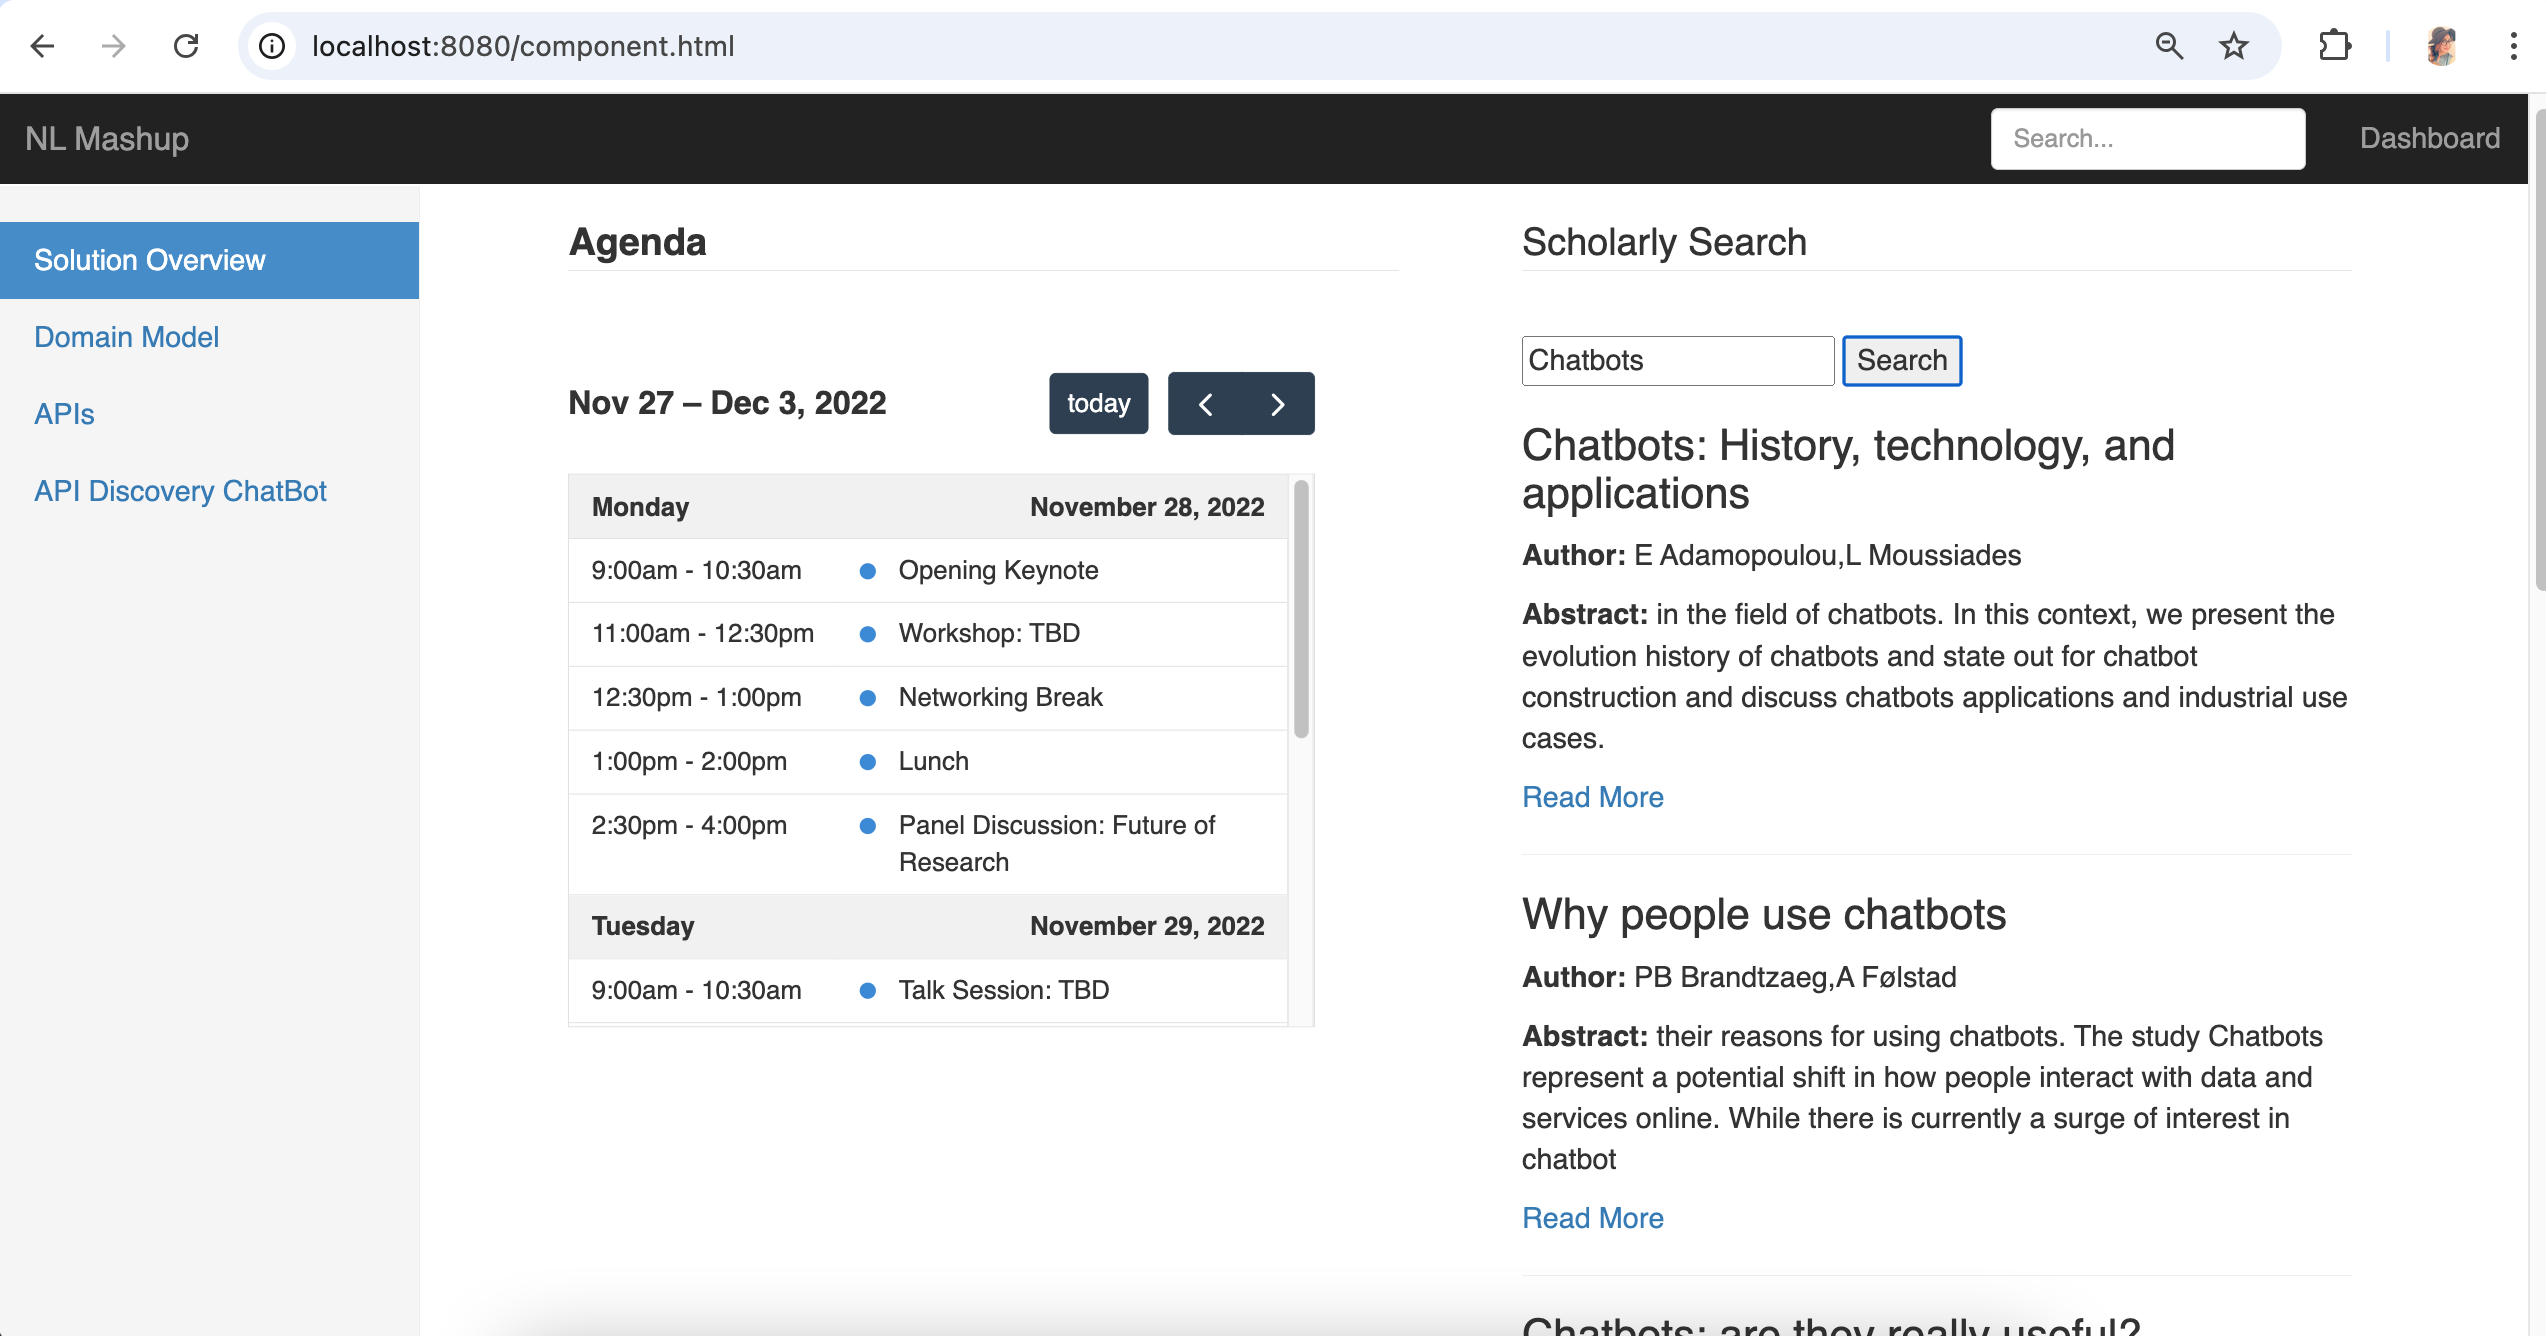
\includegraphics[width=0.85\textwidth]{../figures/MyFigures/event-planner.png}
\captionsetup{justification=centering}
\caption{Event Planning Use Case Application}\label{fig:eval-planning}
}
\end{figure}

\vspace{-15pt}
\hypertarget{sec:evaluation.scenario-gowda}{%
\subsection{Goal-oriented Web Document Querying Tool (GoWDa)}\label{sec:evaluation.scenario-gowda}}
\vspace{15pt}
The ontology generator component enhances the web documents querying with a focus on domain specificity. GoWDa, a goal-oriented web documents querying tool presented in \autocite{Zarei2018} and discussed as part of the ACM Symposium on Document Engineering. This tool generates the domain ontology and enables users to run queries on web documents. The queries are mapped onto the goal ontology to extract goal and objective hierarchies. This mapping enhances the query interpretation and context awareness. Then GoWDa uses the domain ontology to semantically annotate web documents using RDF syntax and run goal-oriented queries on these annotations. Although the LLMs were not truly introduced when publishing this paper, they can be easily integrated into the ontology generator component and enhance the result’s precision. The GoWDa can be a standalone component for E-learning platforms, educational chatbots, and Enterprise Knowledge Management tools.


\vspace{-15pt}
\hypertarget{sec:evaluation.summary}{%
\section{Summary}\label{sec:evaluation.summary}}
\vspace{15pt}

In this section, a comprehensive evaluation of the DSAC approach is presented, by assessing the methodology and toolkit. Although the tools and mechanisms within the DSAC framework were evaluated individually in previous chapters, this chapter focuses on assessing the framework as a whole and comparing this approach to existing solutions discussed in \cref{sec:sota}. The analysis showed full satisfaction with development process requirements and tool requirements except for Functionality Integration, and Interactive User Interface which were partially satisfied. This stems from the deliberate choice to put effectiveness and usability first by separating responsibility based on the skillsets. Additionally, this chapter includes scenarios demonstrating the implementation of DSAC platform and its toolkits to underscore its feasibility. 